\documentclass[11pt, a4paper]{article}
\usepackage[utf8]{inputenc}
\usepackage{fancyhdr}
\usepackage{graphicx}
\PassOptionsToPackage{hyphens}{url}\usepackage{hyperref}
\usepackage{geometry}
\usepackage[
backend=biber,
style=apa,
]{biblatex}
\usepackage{kotex}

\addbibresource{reference.bib}

\pagestyle{fancy}
\fancyhf{}
\setlength{\headheight}{14pt}
\rhead{Master dissertation}
\lhead{sukhoon park}
\cfoot{\thepage}

\begin{document}

\title{AI Report}
\author{Siyun Min}
\maketitle

\tableofcontents

\section{중산층 개념 논의}
중산층 관련 발표를 하는걸로. 지도교수 컨펌 필요. 이론적으로 쓰고 그걸 학위논문화시키고 다시 요약본과 분석을 논문으로 재생산하는 것. \\

한국에서의 중산층 개념은 개념 속 중의 의미가 객관적인지 중산층인지에 따라 중위소득을 기준으로한 객관적 개념과 개인이 그러하다고 느끼는 주관적 계층의식(subjective social status) 개념으로 구분된다(reference). 그 중 전자는 학자들() 사이에서 계급(class)이라는 용어와 혼용해서 사용된다. 강희경(2016)은 사회과학자들이 제시한 ₩주관적 계층의식'개념이 실제 계급에 기반한 정치 투표 행태를 설명하지 못한다고 비판한다. \\

홍두승(2005)은 한 사람을 중산층으로 직업, 소득, 자산, 교육, 중산층 귀속의식을 제시하였다. 

홍두승. (2005). 한국의 중산층 = (The)Middle Classes in Korea / 홍두승 저.

최민호. (2018). 지역사회의 자본요인에 대한 평가가 삶의 질에 미치는 영향 - 주관적 계층의식의 조절효과를 중심으로.

어떤 것을 통제하였는가?  사회조사 3개년도 설문지. 중산층 연구 토

\subsection{객관적 계급?}

\subsection{주관적 계층의식}



\section{MDIS, 행정데이터를 통해서 분석}


\subsection{한국에서의 중산층이란?}

\subsection{중민이론, 한상진, 김홍중}

\subsection{해외 중산층 논의}

\section{한국적인 상황}

\subsection{위험사회, 위험 바라보는 두 가지 시각들}

\subsection{학자 정리. 이재열, 홍두승, 장경섭.}

\subsection{장경섭에서 부모 부양이라는 것을 끄집어 내는 것.}

\section{국민이전계정}
\subsection{통계청 발표 자료 참고+Manual(확보완료)}
\subsection{데이터 요청해서 받고 기초분석. 지역별로? RDC}

\section{실제분석}
\subsection{네트워크?}
\subsection{들어간 기초자료}
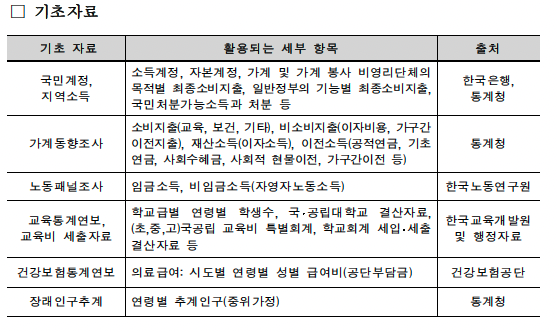
\includegraphics[]{basic_material_list.png}



\printbibliography

\end{document}